%%%%%%%%%%%%%%%%%%%%%%%%%
%% Header for standard beamer presentation
%%
%%  PresentationHeader.tex
%%
%%%%%%%%%%%%%%%%%%%%%%%%%

\documentclass[english,10pt]{beamer}

%%%%%%%%%%%%%%%%%%%%
%% Include general header where common packages are defined
%%%%%%%%%%%%%%%%%%%%

% general packages without options
\usepackage{amsmath,amssymb,bbm}




%%%%%%%%%%%%%%%%%%%%
%% Idem general commands
%%%%%%%%%%%%%%%%%%%%

%%% Commands

\newcommand{\noun}[1]{\textsc{#1}}


%% Math

% Operators
\DeclareMathOperator{\Cov}{Cov}
\DeclareMathOperator{\Var}{Var}
\DeclareMathOperator{\E}{\mathbb{E}}
\DeclareMathOperator{\Proba}{\mathbb{P}}

\newcommand{\Covb}[2]{\ensuremath{\Cov\!\left[#1,#2\right]}}
\newcommand{\Eb}[1]{\ensuremath{\E\!\left[#1\right]}}
\newcommand{\Pb}[1]{\ensuremath{\Proba\!\left[#1\right]}}
\newcommand{\Varb}[1]{\ensuremath{\Var\!\left[#1\right]}}

% norm
\newcommand{\norm}[1]{\| #1 \|}


% amsthm environments
\newtheorem{definition}{Definition}



%% graphics

% renew graphics command for relative path providment only ?
%\renewcommand{\includegraphics[]{}}






\usetheme{Warsaw}

\setbeamertemplate{footline}[text line]{}
\setbeamercolor{structure}{fg=purple!50!blue, bg=purple!50!blue}

\setbeamercovered{transparent}


% shortened command for a justified frame
\newcommand{\jframe}[2]{\frame{\frametitle{#1}\justify{#2}}}



%%%%%%%%%%%%%%%%%%%%%
%% Begin doc
%%%%%%%%%%%%%%%%%%%%%

\begin{document}



\title{Thesis Progress Meeting}


\author{J.~Raimbault$^{1,2}$}

\institute{$^{1}$G{\'e}ographie-cit{\'e}s (UMR 8504 CNRS)\\
$^{2}$LVMT (UMR-T 9403 IFSTTAR)}


\date{January 26th 2016}


%%%%%%%%%%%%%%%%%%%%%%%%%%%%%%%%
\begin{frame}
\titlepage
\end{frame}

%\begin{frame}
%\tableofcontents
%\end{frame}
%%%%%%%%%%%%%%%%%%%%%%%%%%%%%%%%


%\section{Projects Organization}

%\jframe{Projects Organization}{
%   \includegraphics[width=\textwidth,height=0.8\textheight]{figures/orgaProjects}
%}



\section{Achieved Work}


\jframe{Achieved Work (by projects)}{
\begin{itemize}
\item Biblio/Meetings/Organisation [0.7w]
\item Conference [0.7w]
\item Reading Records (\emph{Synergetics}~\cite{sanders1992systeme}) [0.2w]
\item Monitorat [1,3w]
\item Cybergeo Project [1w]
\item Correlated Synthetic data [3w]
\item Theory construction (communication JIG) [0.2w]
\item BP Case Study / Spatial Econometrics [0,3w]
\end{itemize}

}



\section{Correlated Synthetic Data}

\sframe{Context}{

\textit{\small[Introduction at Rochebrune] : imagine a model of simulation describing skiers/ snowboarders relations, measures to improve situation ? NO conclusion without model exploration, including sensitivity to ressort station spatial configuration, or to population structure, even at second order $\rightarrow$ Necessity in that case (among others) to generate synthetic data controlled at second order.}


\bigskip

\textbf{Def. : } \emph{Synthetic Data} are output of generative models (and possibly inputs of models using them).
\medskip

Methodology used in various fields, e.g. therapeutic evaluation~\cite{abadie2010synthetic}, territorial systems analysis~\cite{moeckel2003creating,pritchard2009advances}, machine learning~\cite{bolon2013review} or bio-informatics~\cite{van2006syntren}.

\medskip

Few examples at the second order : specific examples as~\cite{ye2011investigation} for discrete choices ; methods that can be interpreted this way : generation of complex networks~\cite{newman2003structure}.

}



%%%%%%%%%%%%%%%%%
\sframe{Generic Method}{
$\vec{X}_I$ multidimensional stochastic process, $\mathbf{X}=(X_{i,j})$ realizations. 

\bigskip

\textbf{Aim : } Generate a statistical population $\mathbf{\tilde{X}}=\tilde{X}_{i,j}$ such that:
\medskip
\begin{enumerate}
\item proximity to data : given a precision $\varepsilon$ and an indicator $f$, $\norm{f(\mathbf{X})-f(\mathbf{\tilde{X}})} < \varepsilon$
\item control of the estimated correlation structure : $\hat{\Var{}}\left[(\tilde{X}_i)\right] = \Sigma R$ with $R$ fixed.
\end{enumerate}

}


%%%%%%%%%%%%%%%%%
\sframe{Geographical data : Context}{

\begin{itemize}
\jitem{In geography, generation of synthetic populations for agent-based models~\cite{pritchard2009advances}.}
\jitem{Generation of spatial synthetic configuration not used (Geo. Weighted Regression~\cite{brunsdon1998geographically} can be interpreted this way) ; however crucial for abstract models~\cite{schmitt2014modelisation}}
\jitem{\cite{cottineau2015revisiting} recently proposed to estimate the sensitivity of spatial models of simulation to initial configuration (application to Schelling model).}
\jitem{Case study : city-transportation interactions, complex to understood quantitatively~\cite{offner1993effets,bretagnolle:tel-00459720} $\rightarrow$ simple model of population density and transportation network morphogenesis.}
\end{itemize}
}



%%%%%%%%%%%%%%%%%
\sframe{Model}{
\footnotesize
Simple coupling between
\begin{itemize}
\jitem{Iterative generation of a density grid by preferential attachment/diffusion~\cite{raimbault2016calibration},  calibrated on morphological objectives on european density grid.}
\jitem{Heuristic network generation conditional to density :
\begin{itemize}
\footnotesize
\item Distribution of a fixed number of centers preferentially following density
\item Deterministic percolation between closest neighbors
\item Breaking of interaction potentials
\[
V_{ij}(d) = \left[ (1 - k_h) + k_h \cdot \left( \frac{P_i P_j}{P^2} \right)^{\gamma} \right]\cdot \exp{\left( -\frac{d}{r_g (1 + d/d_0)} \right)}
\]
for a fixed number of couples $N_L$ such that $V_{ij}(d_N)/V_{ij}(d_{ij})$ is minimal among $K\cdot N_L$ strongest euclidian potentials ($K=5$ fixed)
\item Planarization
\end{itemize}
}
\end{itemize}
Indicators : morphology~\cite{le2015forme} (Moran, mean distance, entropy, hierarchy) and network (centrality, mean width, speed, diameter).

}

%%%%%%%%%%%%%%%%%
\sframe{Implementation and Exploration}{

$\rightarrow$ Formal and Operational coupling : modular implementation (\texttt{scala}/\texttt{NetLogo}) encapsulated by \texttt{OpenMole}~\cite{reuillon2013openmole}

\bigskip

$\rightarrow$ Exploration by intensive computation on grid via \texttt{OpenMole} : calibration of density model alone ($\sim 1.5\cdot 10^6$ runs) ; brutal exploration by LHS sampling for feasible correlations ($\sim 5\cdot 10^4$ runs) 

}



%%%%%%%%%%%%%%%%%
\sframe{Results : Density Model alone}{
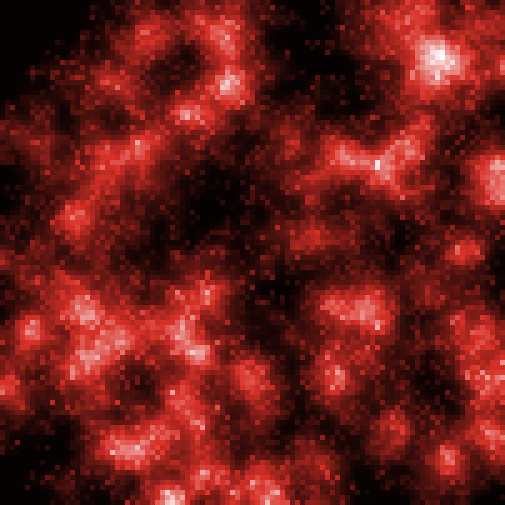
\includegraphics[width=0.24\textwidth]{figures/density/conf1}\hspace{0.1em}
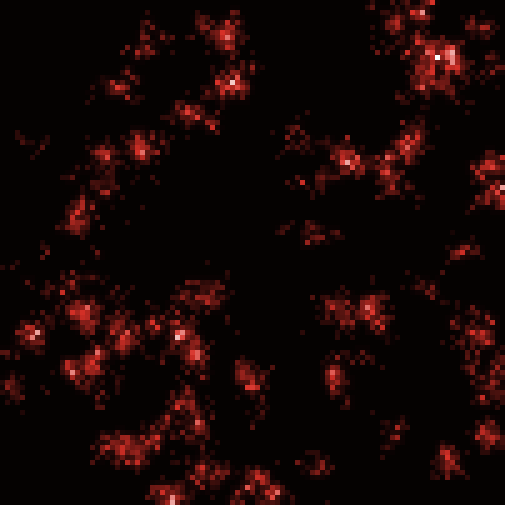
\includegraphics[width=0.24\textwidth]{figures/density/conf2}\hspace{0.1em}
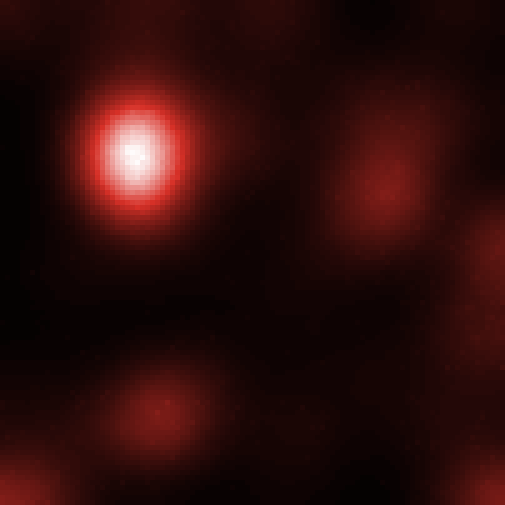
\includegraphics[width=0.24\textwidth]{figures/density/conf3}\hspace{0.1em}
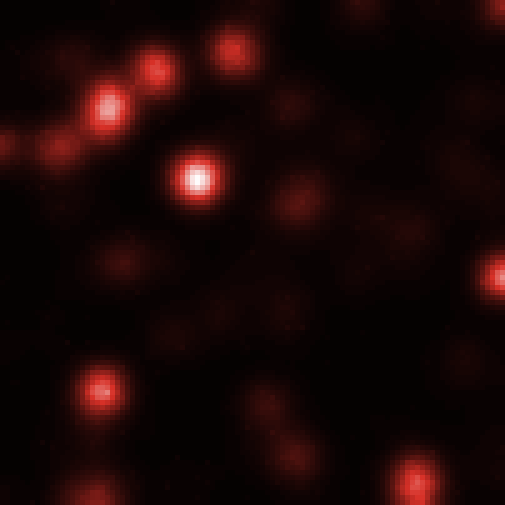
\includegraphics[width=0.24\textwidth]{figures/density/conf4}\hspace{0.1em}
\\
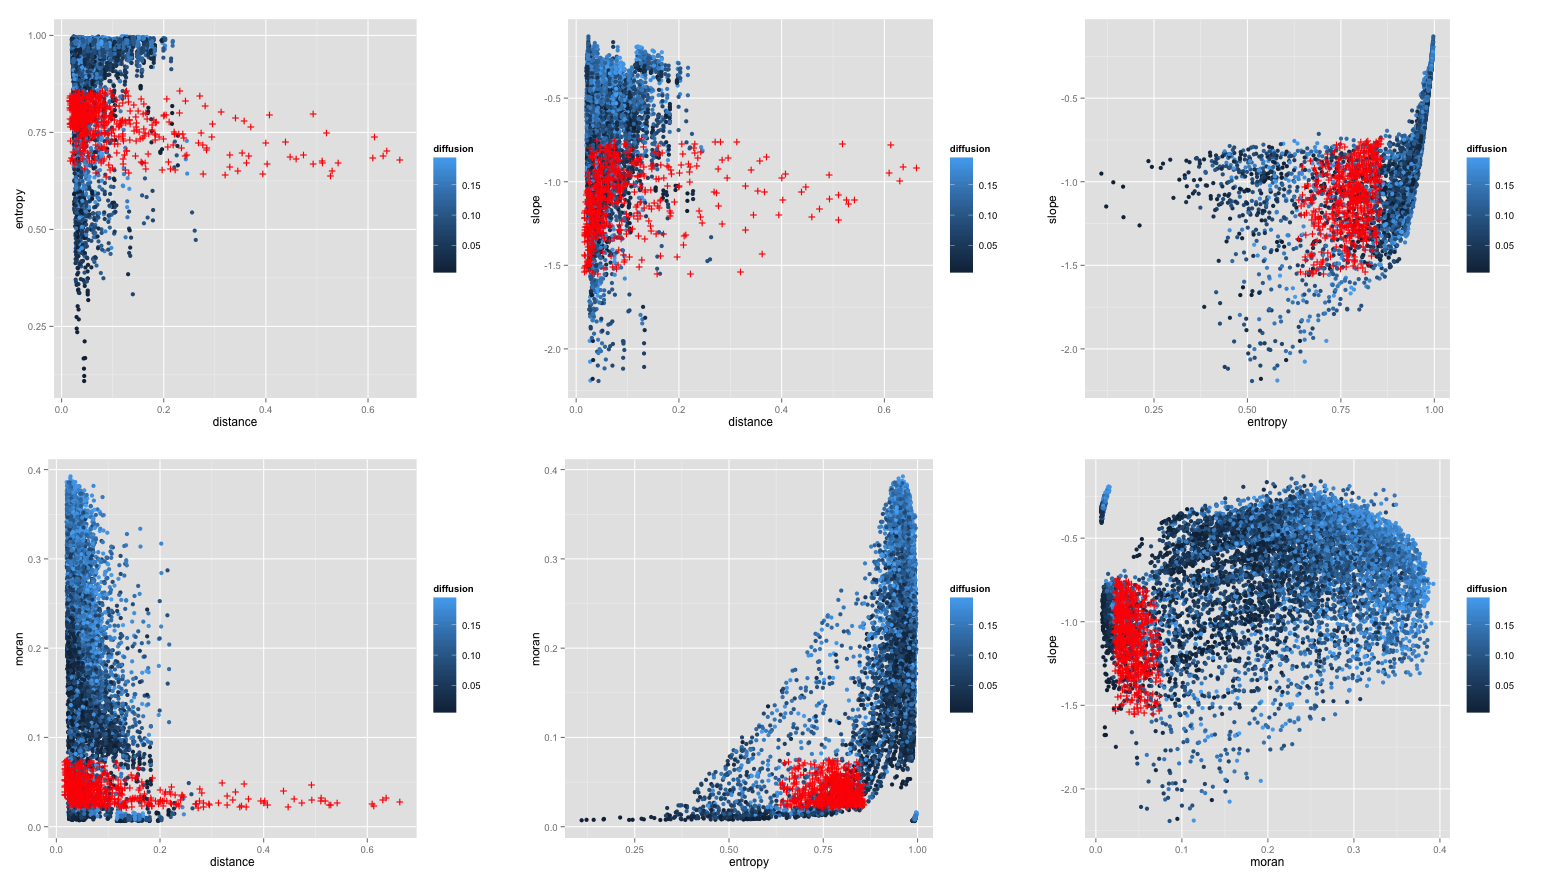
\includegraphics[width=0.5\textwidth,height=0.55\textheight]{figures/density/scatt}
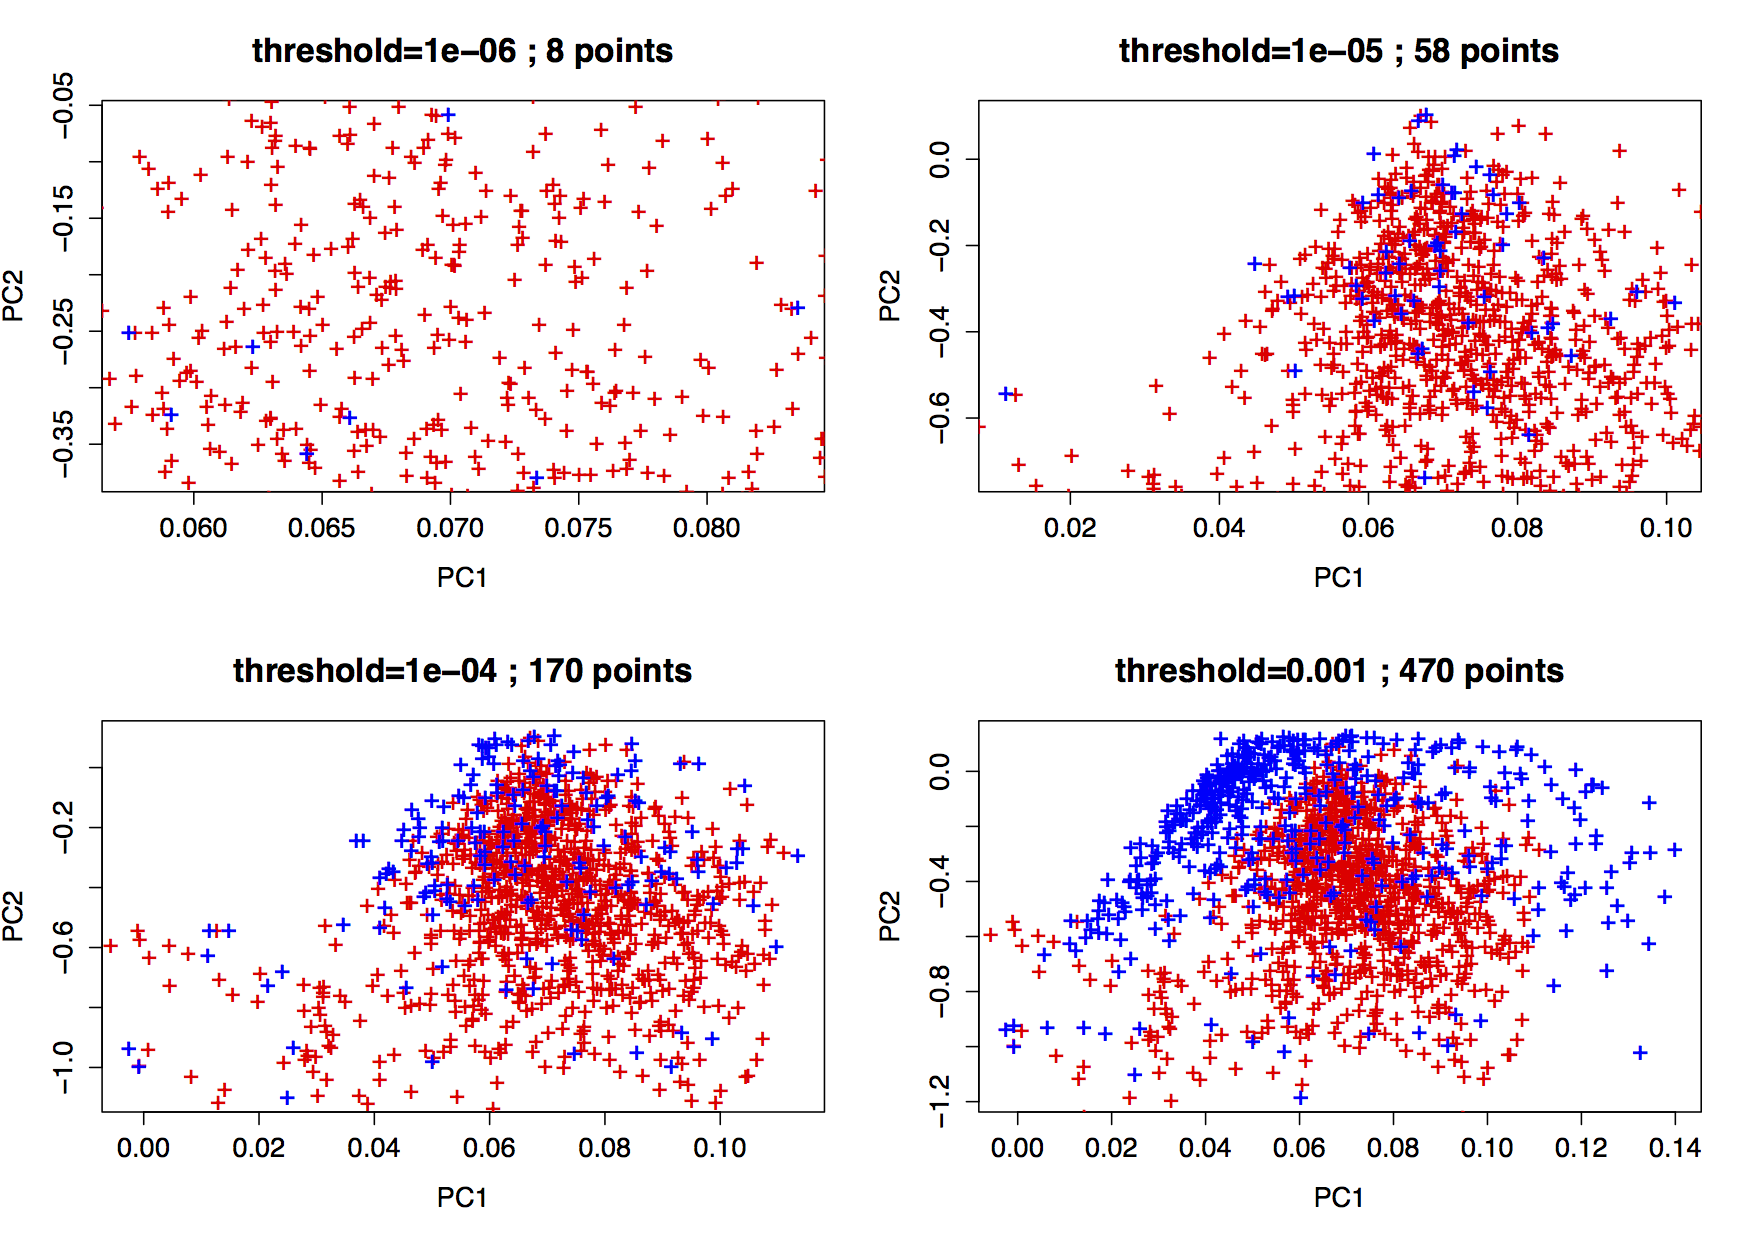
\includegraphics[width=0.5\textwidth,height=0.55\textheight]{figures/density/pca}
}



%%%%%%%%%%%%%%%%%
\sframe{Results : examples of configurations}{
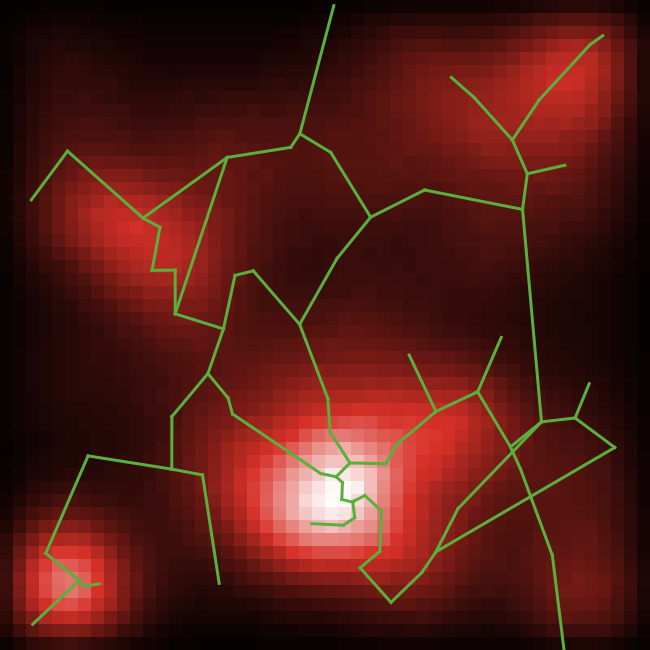
\includegraphics[width=0.49\textwidth]{figures/configs/2_param71913_seed10}\hspace{0.1cm}
   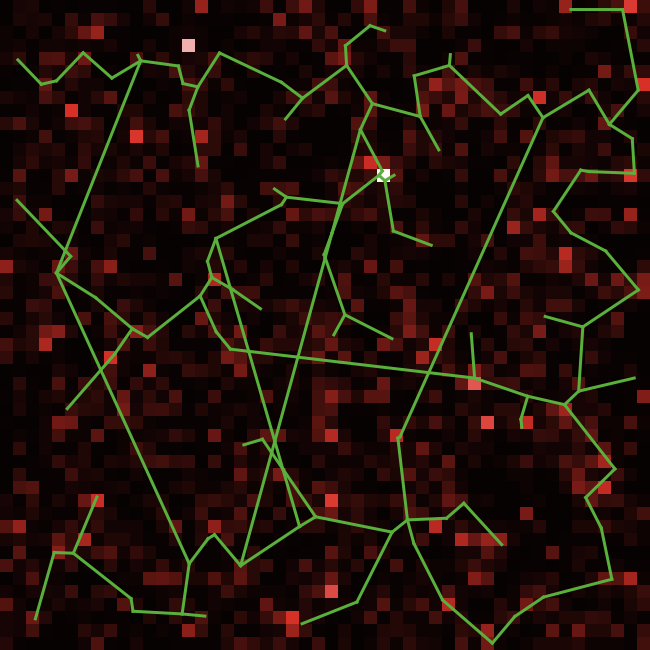
\includegraphics[width=0.49\textwidth]{figures/configs/3_param71918_seed0}
}

%%%%%%%%%%%%%%%%%
\sframe{Results : examples of configurations}{
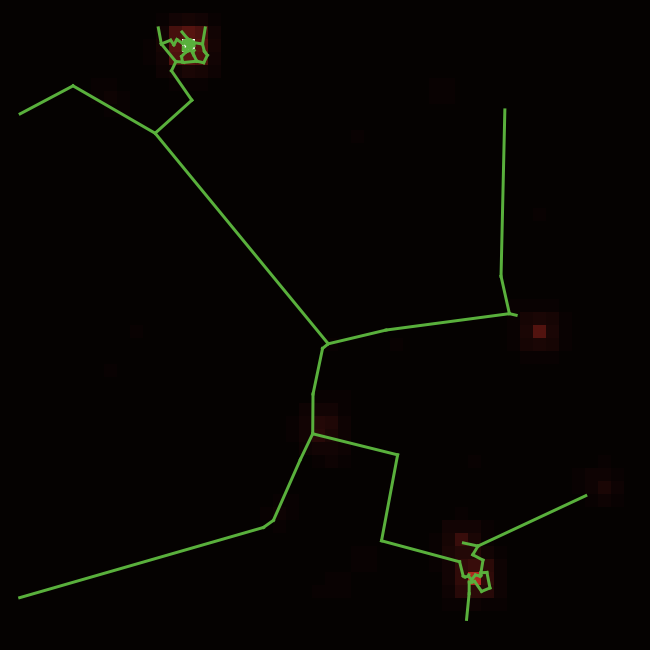
\includegraphics[width=0.49\textwidth]{figures/configs/1_param71861_seed0}\hspace{0.1cm}
   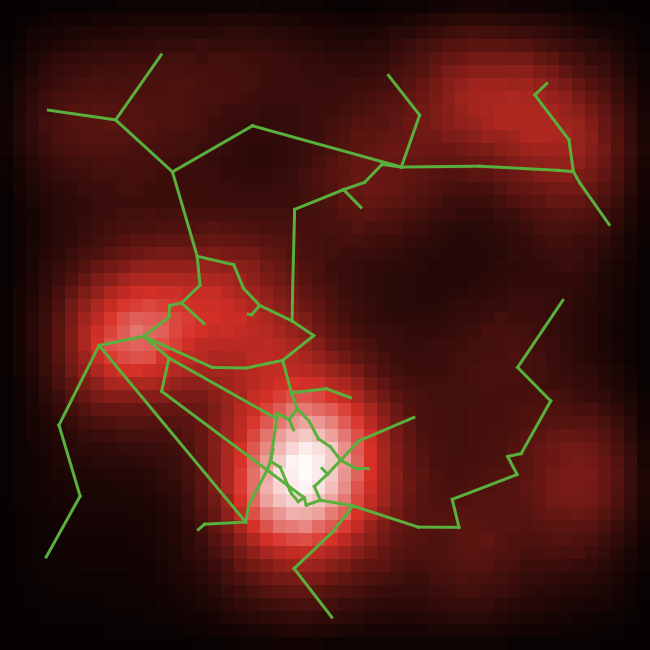
\includegraphics[width=0.49\textwidth]{figures/configs/4_param71945_seed0}
}




%%%%%%%%%%%%%%%%%
\sframe{Results : cross-correlations}{
\centering
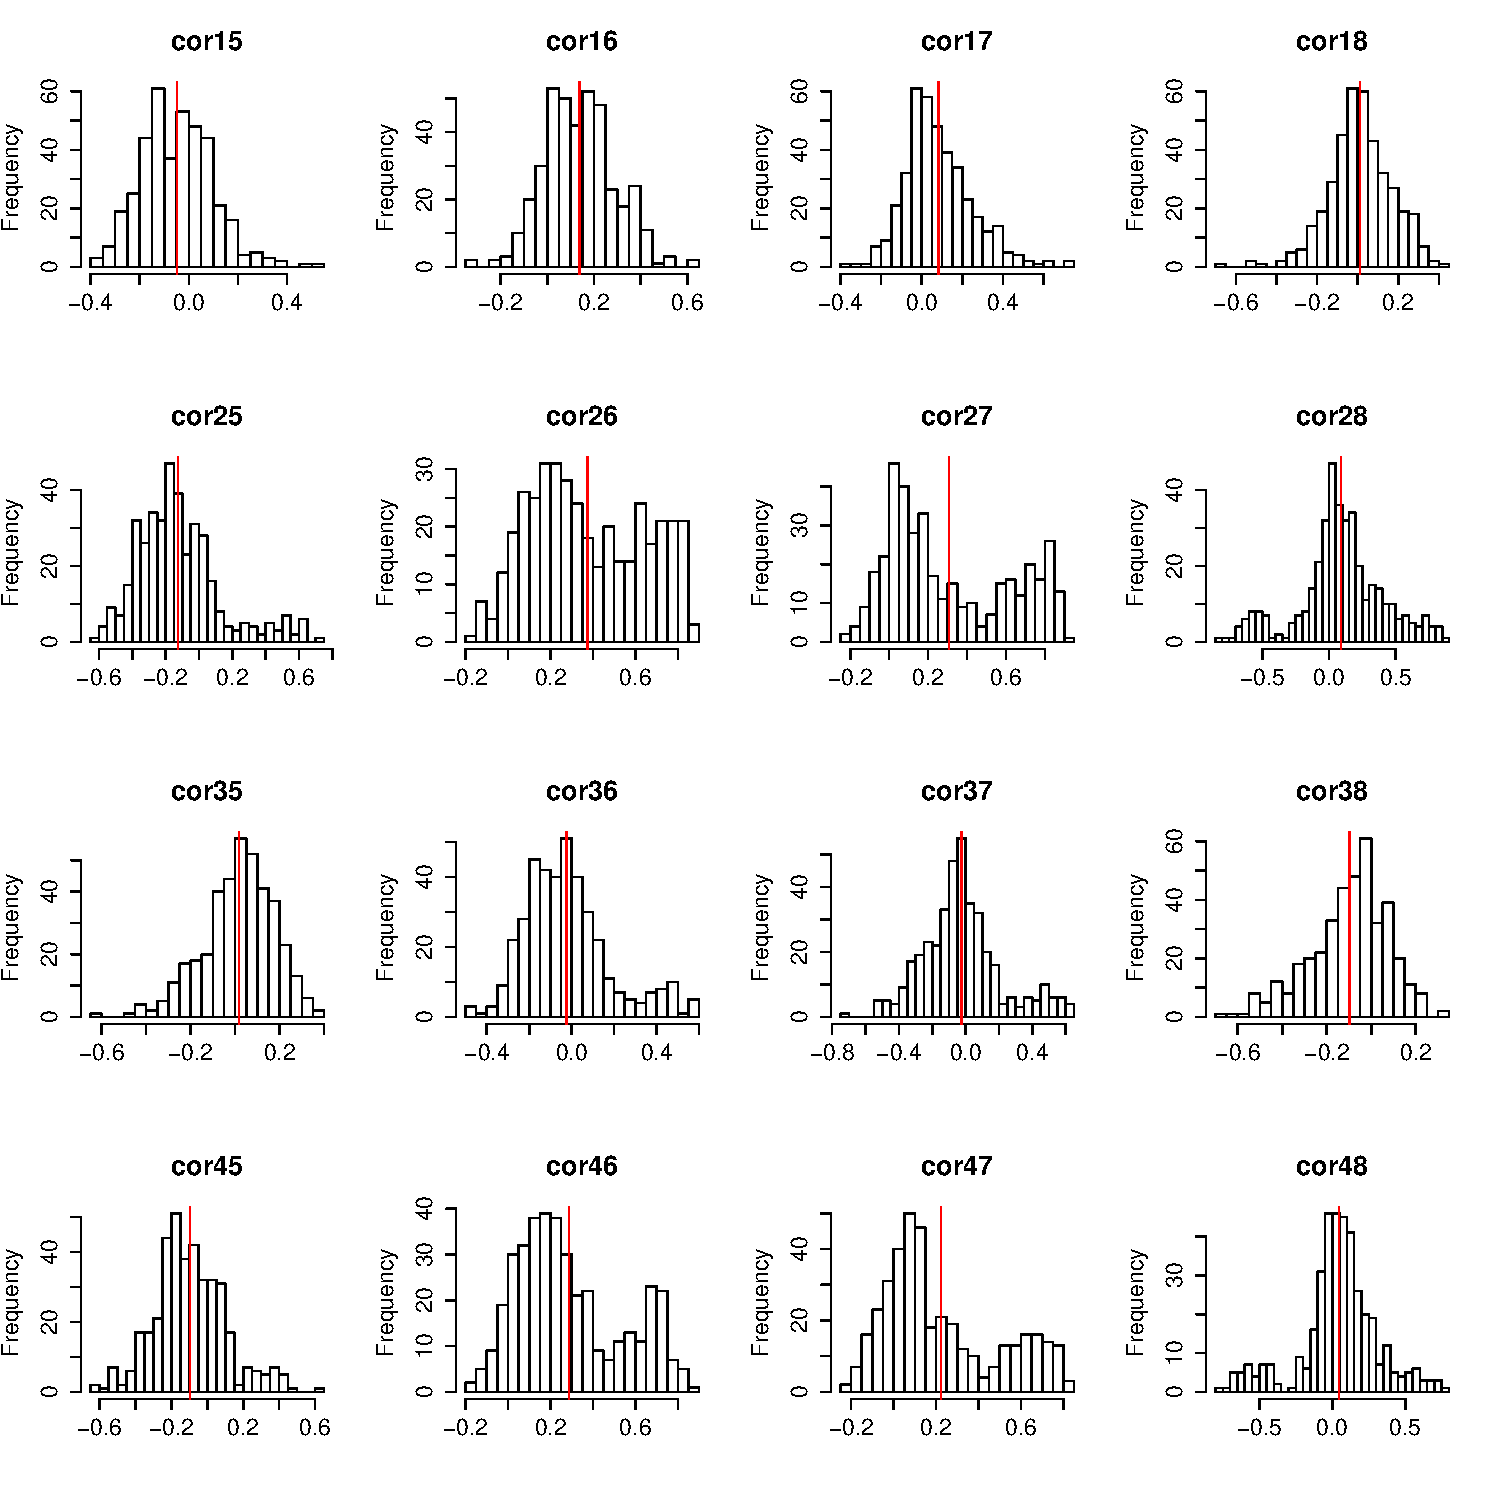
\includegraphics[height=0.85\textheight]{figures/hist_crossCorMat_breaks30}
}

%%%%%%%%%%%%%%%%%
\sframe{Results : feasible correlations}{
\textit{Mean matrices in a principal plan}

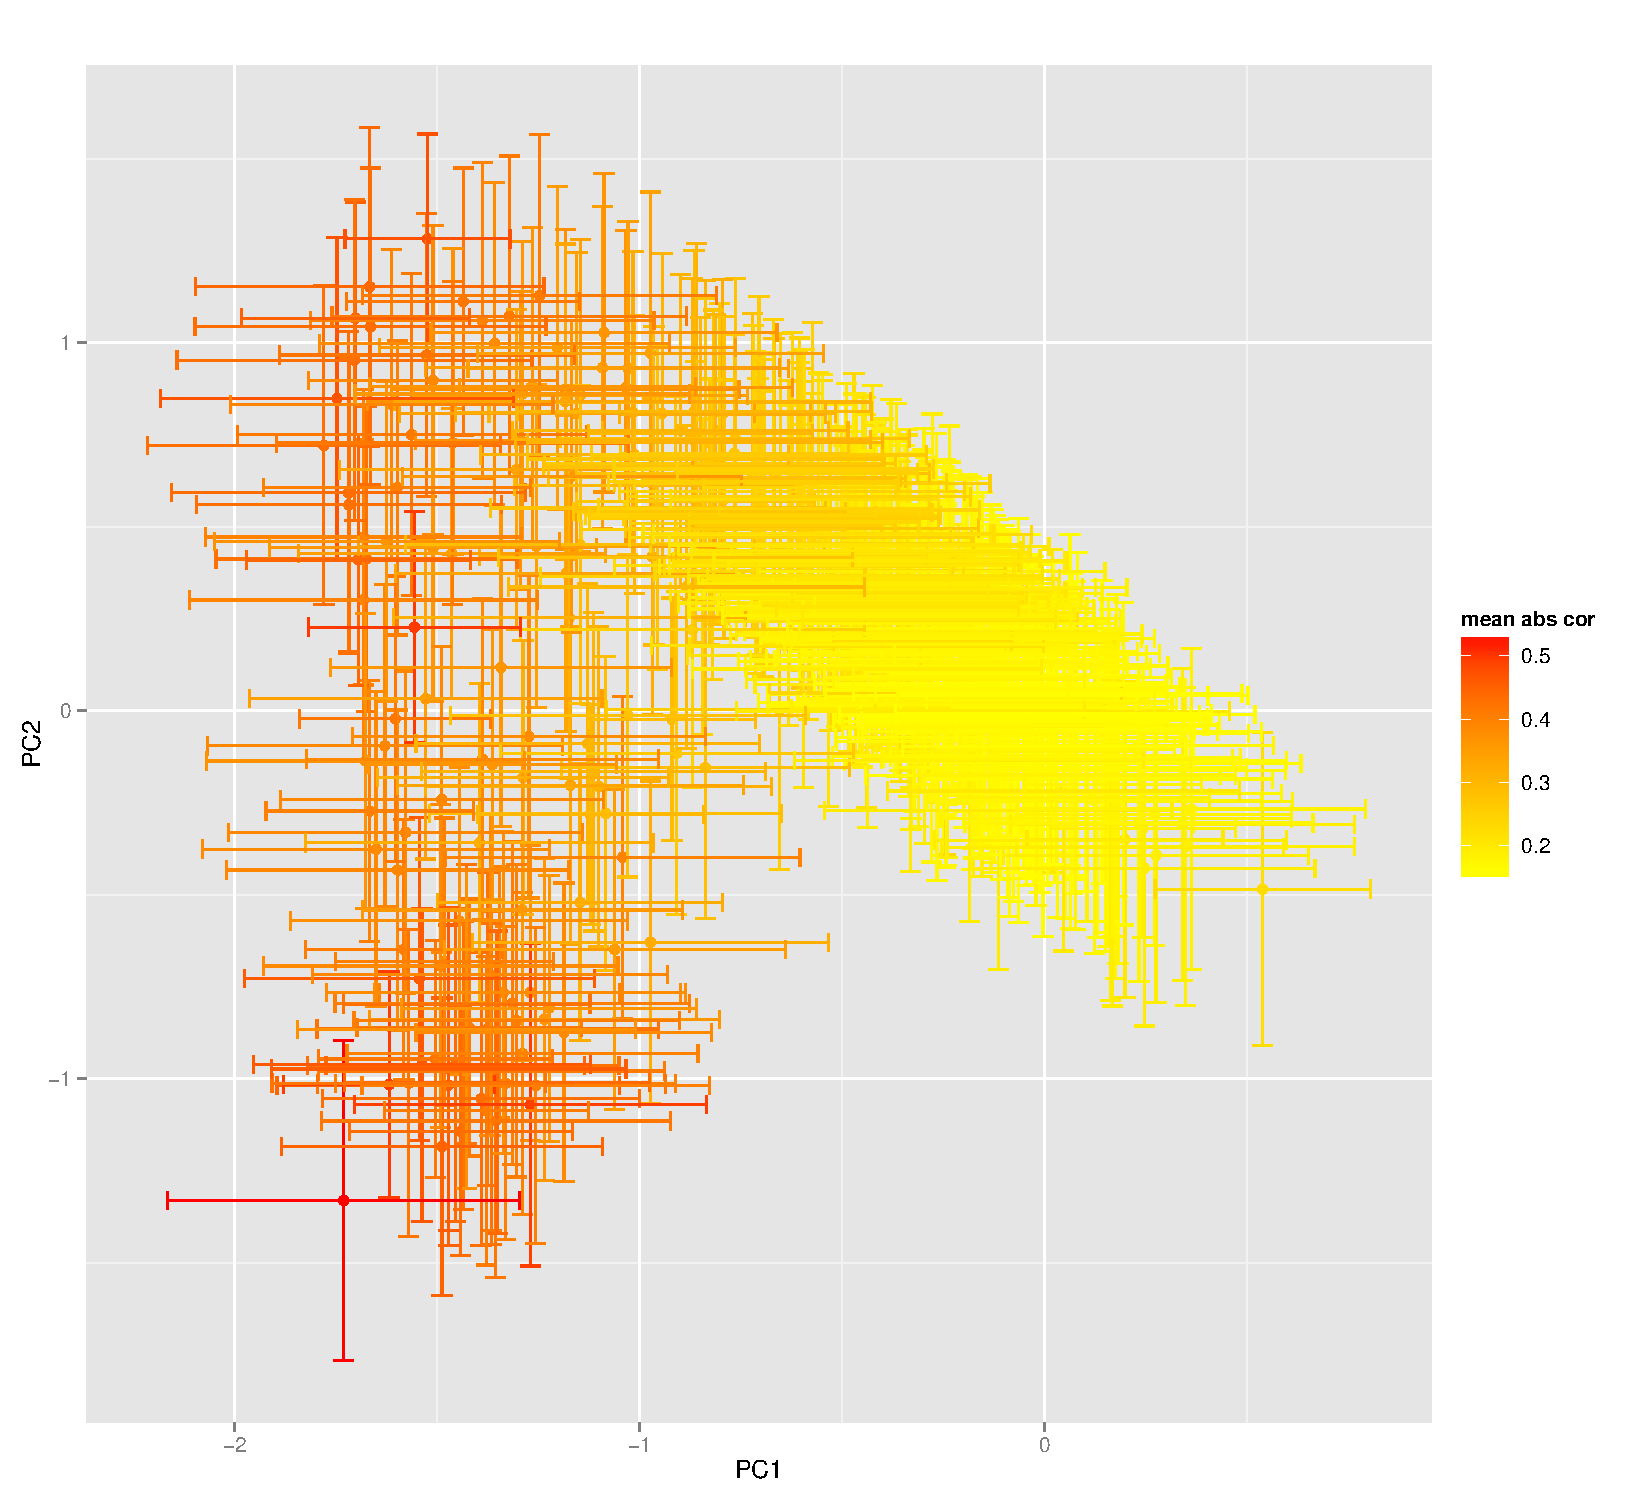
\includegraphics[width=0.5\textwidth,height=0.65\textheight]{figures/pca_meanAbsCor_errorBars}
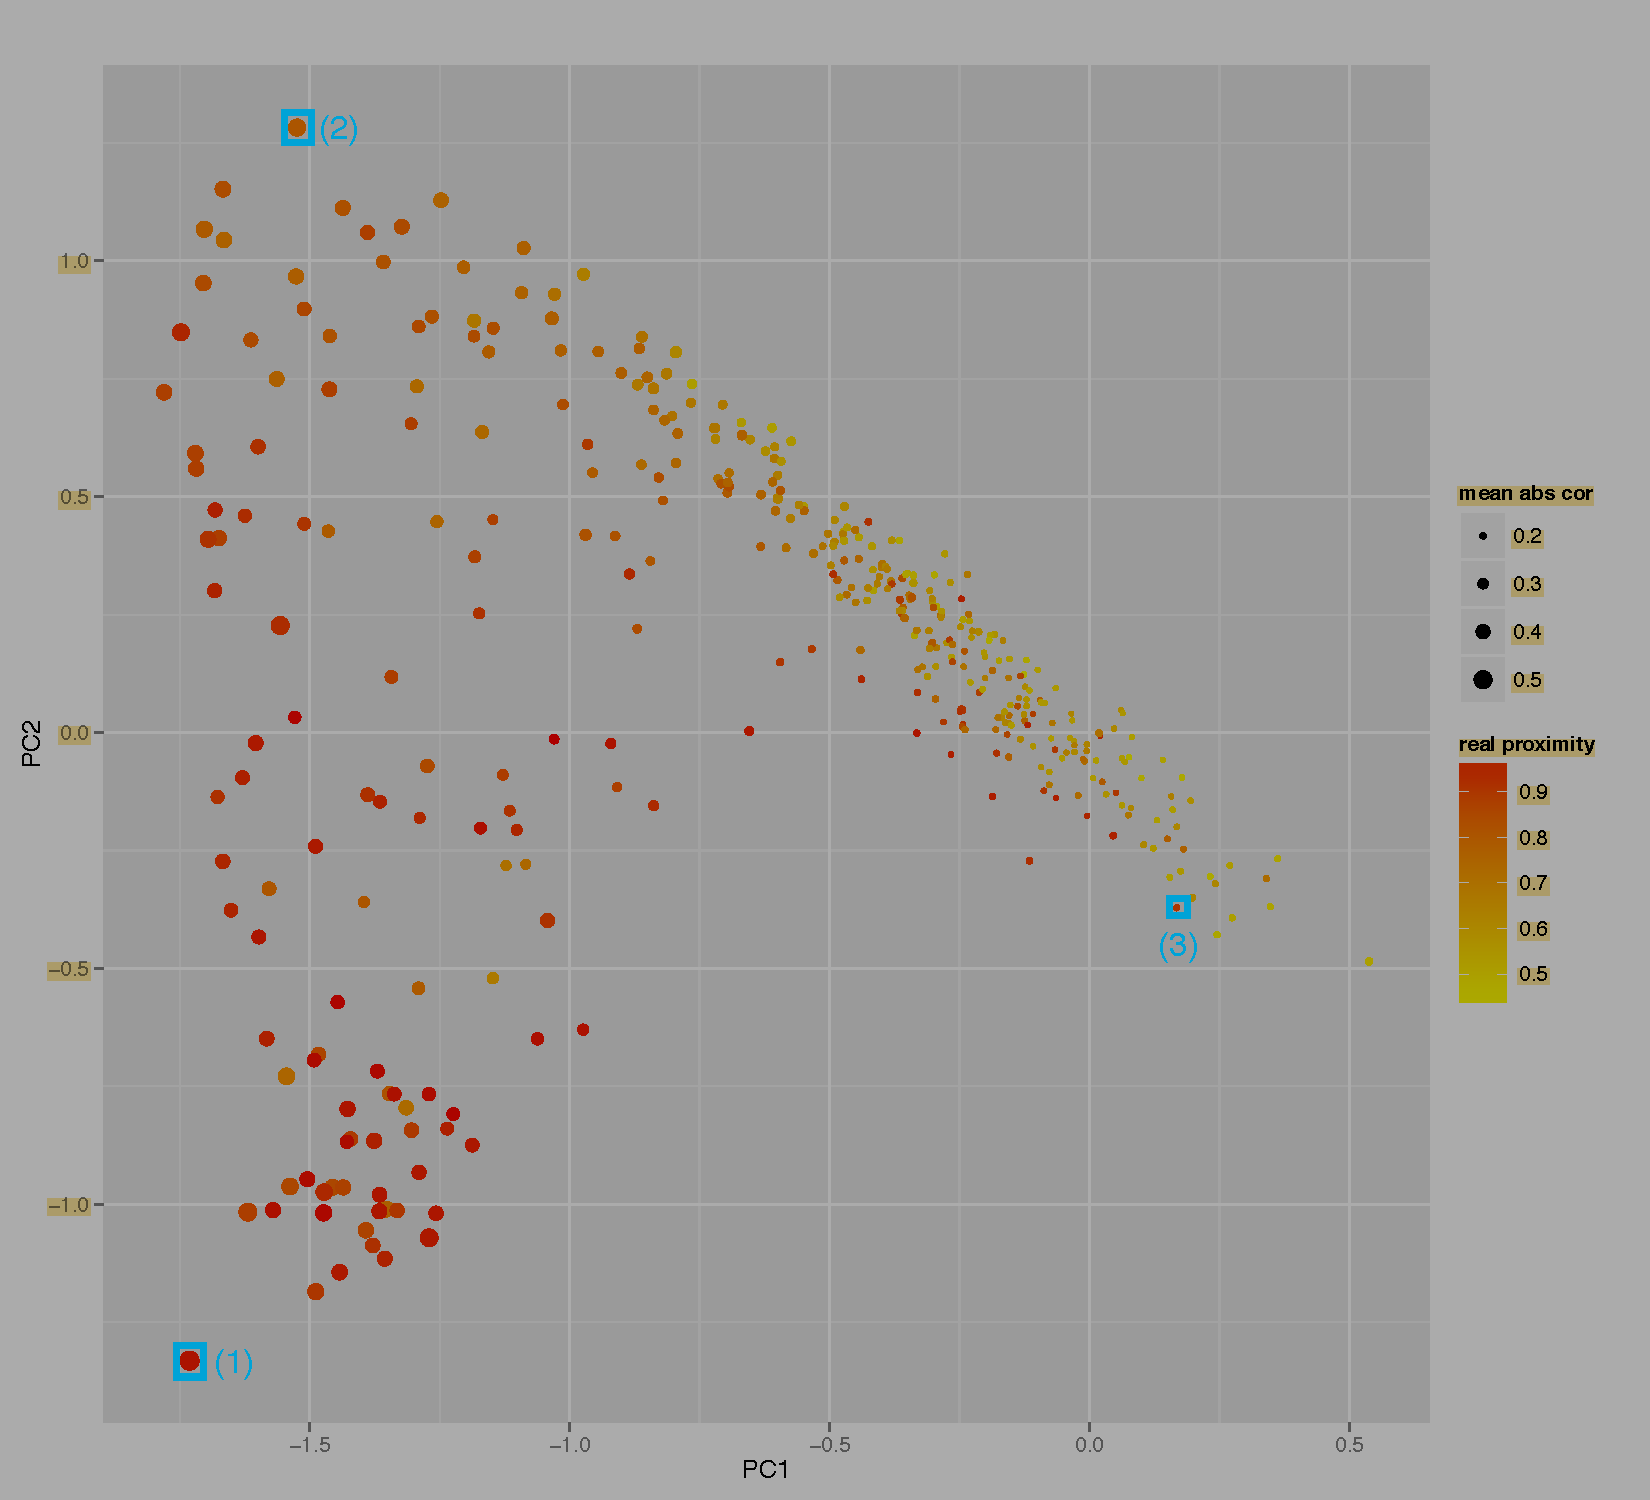
\includegraphics[width=0.5\textwidth,height=0.65\textheight]{figures/pca_realDistCol_meanAbsCorSize_withSpecificPoints}
}

%%%%%%%%%%%%%%%%%
\sframe{Results : exemples of correlations}{
\begin{columns}[T] % align columns
\begin{column}{.48\textwidth}
\centering
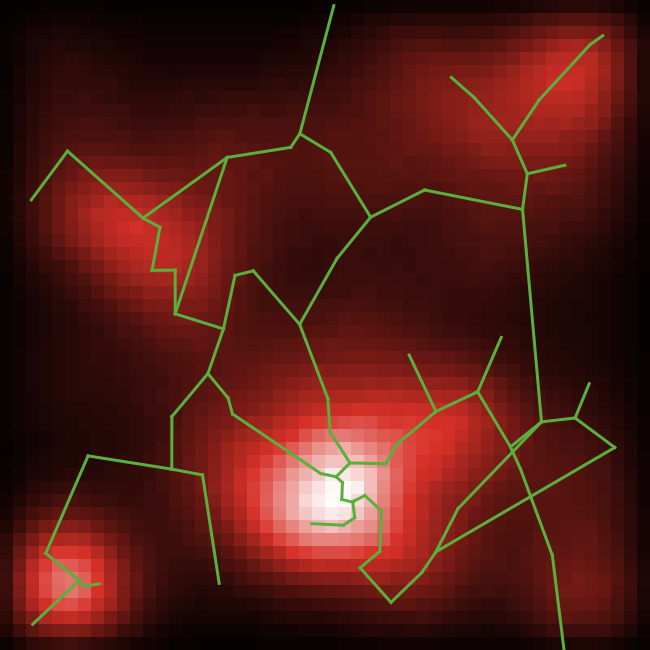
\includegraphics[width=\textwidth]{figures/configs/2_param71913_seed10}\\
$\rho[\bar{d},\bar{c}]\simeq 0.34$
\end{column}%
\hfill%
\begin{column}{.48\textwidth}
\centering
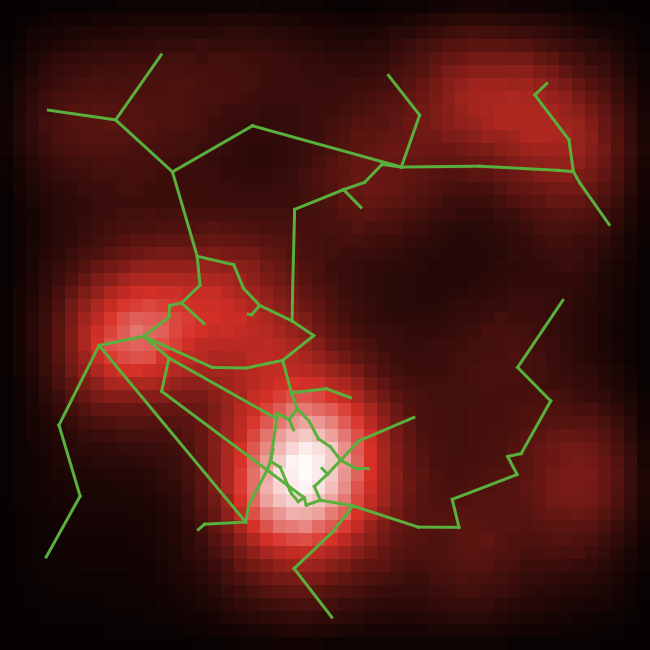
\includegraphics[width=\textwidth]{figures/configs/4_param71945_seed0}\\
$\rho[\bar{d},\bar{c}]\simeq-0.41$
\end{column}%
\end{columns}

$\rightarrow$ \textit{gravity hierarchy more important in (1) $\gamma=3.9,k_h=0.7$ against $\gamma=1.07,k_h=0.25$ for (2)}

}



%%%%%%%%%%%%%%%%%
\sframe{Applications}{

\begin{enumerate}
\item Calibration of the coupled model, street network data (¡ edge effects!)\\$\rightarrow $ generation of correlated synthetic data corresponding to a given urban system\\$\rightarrow$ intrinsic correlations to be compared to estimated correlations between different states : non-ergodicity of urban systems~\cite{pumain2012urban}).
\bigskip
\item Dynamical correlations in a strongly coupled model / spatio-temporal correlations in a strong spatial coupling.
\end{enumerate}

}


\section{Spatial Statistics}

\sframe{Case study : Context}{
\textbf{Database by Florent : } main road network (route 120) in extended \emph{Bassin Parisien} with opening dates for highways ; census data : population and employment of \emph{communes} at dates [other data such as rail network and train timetables not used for now].

\bigskip

\textbf{Formalisation : } Dynamic transportation network $n(\vec{x},t)$ within a dynamic territorial landscape $\vec{T}(\vec{x},t)$, which components are population $p(\vec{x},t)$ and employments $e(\vec{x},t)$, discretized in space and in time, i.e. the spatial field $\vec{T}$ is summarized by $\mathbf{T} = \left(\vec{T}(\vec{x}_i,t_j)\right)_{i,j}$ with $1\leq i \leq N$ and $1\leq j \leq T$. To simplify, network distances sampled at same times and spatial points (support extended if not the case), given by $\mathbf{N} = \left(\vec{d}_n(\vec{x}_i,t_j)\right)_{i,j}$.



}


\sframe{On Accessibility}{

\textit{\textbf{Is the notion of accessibility crucial for statistical analysis ?}}

\medskip

\footnotesize

Weibull has proposed an axiomatic approach to accessibility~\cite{weibull1976axiomatic}, deriving a canonical decomposition for any \emph{attraction-accessibility} function $A(a,d)$, assuming expected thematic axioms among others technical ones that are :
\begin{enumerate}
\item \footnotesize $A$ is invariant regarding the order of the configuration
\item \footnotesize $A$ decrease with distance at fixed attraction and increase with attraction at fixed distance
\item \footnotesize $A$ is invariant when adding null attractions and constant configurations
\end{enumerate}
Then $A$ verifies these \emph{iff} it is of the form
\[
A\left[(a_i,d_i)\right] = T\left(\bigoplus_i z(d_i,a_i)\right)
\]
where $T$ is increasing with null origin, $z$ is a \emph{distance substitution function} (i.e. verifying axiom 2) and $\oplus$ a \emph{standard composition} associating two attractions at zero distance to th corresponding unique one. 

$\rightarrow$ \textit{Well suited matrices of autocorrelation should capture accessibility in regressions ; or captured by non-linear regression on $\mathbf{N}$}

\medskip

{\normalsize\textit{\textbf{Accessibility as potential ?}}}

Given any stationary dynamic for $n,\vec{T}$, Helmoltz theorem states that it derives from a potential (can be adapted to non-stationary dynamics with time-varying potential).

}

\sframe{Statistical Analysis}{
{\small
\textit{Large set of analysis to be tested (non exhaustive) :}
\begin{itemize}
\item On data :
\begin{itemize}
\item Multivariate models $\mathcal{L}\left[\mathbf{T},\mathbf{N}\right]\sim \varepsilon$
\item Autocorrelated univariate models $(\mathbf{I} - \Sigma R W) \mathbf{X} \sim \varepsilon$
\item Autocorrelated multivariate models $(\mathcal{L}' - \Sigma R W)\left[\mathbf{T}+\mathbf{N}\right] \sim \varepsilon$
\item Geographically Weighted Regression~\cite{brunsdon1998geographically}
\[
\mathcal{L}\left[\mathcal{G}\left(\mathbf{T},\mathbf{N}\right)\right] \sim \varepsilon
\]
\item Granger causality tests : \cite{xie2009streetcars} use Granger causality to link transit with land-use changes.
\end{itemize}
\item On data returns :
\begin{itemize}
\item Autoregressive multivariate models
\[\mathcal{L}\left[(\Delta \mathbf{T}(t_{j'}))_{j'\leq j},(\Delta \mathbf{N}(t_{j'}))_{j'\leq j}\right] \sim \varepsilon\]
\item Autoregressive autocorrelated multivariate models : idem with spatial autocorrelation term.
\item Synthetic Instrumental Variables : static territory and/or network ?
\end{itemize}
\end{itemize}
}
}





\section{Next Steps}


\sframe{P. Bourgine framework for Complex Adaptive Systems}{

\small

Bourgine has recently developed a framework to extract patterns of Complex Adaptive Systems, using a representation theorem : any discrete stationary process is a \emph{Hidden Markow Model} (Knight, 1975)

Given the definition of a causal state as $\Pb{future | A} = \Pb{future | B}$, the partition of system states induced by the corresponding equivalence relations allows to derive a \emph{Recurrent Network} that is enough to determine next state of the system, as it is a \emph{deterministic} function of previous state and hidden states~\cite{shalizi2001computational} :
\[
(x_{t+1},s_{t+1}) = F\left[(x_t,s_t)\right]
\]

$\rightarrow$ \textit{Estimation of Hidden States and of the Recurrent Function thus captures through deep learning entirely dynamical patterns of the system, i.e. full information on its dynamics and internal processes.}

\medskip

\textbf{Some questions for an application to Geography : }
\begin{itemize}
\item Can the stationarity assumption be tackled through augmentation of system states ?
\item Can heterogeneous and asynchronous data be used to bootstrap long time-series necessary for a correct estimation of the neural network ?
\end{itemize}


}


%%%%%%%%%%%%%%%%%%%%%%%%%%%%%%%%
\jframe{Next steps (until February 15th 2016)}{
\begin{itemize}
\item Theory exemplification, paper finalization  [1w]\medskip
\item Spatial \sout{Econometrics} Statistics / Case study [0.5w]\medskip
\item Cybergeo [0.5w]\medskip
\item Wrap everything within a 1-year Memoire [1w]\medskip
\end{itemize}
}






%%%%%%%%%%%%%%%%%%%%%%%%%%%%%%%%
\begin{frame}[allowframebreaks]
\frametitle{References}
\bibliographystyle{apalike}
\bibliography{/Users/Juste/Documents/ComplexSystems/CityNetwork/Biblio/Bibtex/CityNetwork,biblio}
\end{frame}
%%%%%%%%%%%%%%%%%%%%%%%%%%%%%%%%


\end{document}